\documentclass[twocolumn,12pt]{article}

\usepackage[utf8]{inputenc}
\usepackage[T1]{fontenc}
\usepackage{lmodern}
\usepackage{microtype}       % improved justification
\usepackage{graphicx}
\usepackage[margin=1in]{geometry}
\usepackage{longtable}
\usepackage{xcolor}
\usepackage{soulutf8}        % utf8-safe highlighting
\usepackage{hyperref}
\usepackage{titlesec}
\usepackage{enumitem}
\usepackage{booktabs}
\usepackage{caption}
\usepackage{amsmath}
\usepackage{float}
\usepackage{fancyhdr}
\usepackage{tcolorbox}       % abstract box
\usepackage{colortbl}        % table row colors
\usepackage{natbib}          % author-year citations

% Hyperref setup
\hypersetup{
    colorlinks=true,
    linkcolor=blue,
    urlcolor=cyan,
    citecolor=blue,
    pdftitle={AI-Powered Methods for Assessing Attention and Focus},
    pdfauthor={},
    pdfstartview=FitH
}

% Colors
\definecolor{teal}{RGB}{0,128,128}
\definecolor{lightgray}{gray}{0.93}

% Section title formatting
\titleformat{\section}{\large\bfseries\color{teal}}{\thesection.}{0.5em}{}
\titleformat{\subsection}{\normalsize\bfseries\color{teal}}{\thesubsection.}{0.5em}{}

% Reduce vertical spacing around sections
\titlespacing*{\section}{0pt}{8pt plus 2pt minus 2pt}{6pt plus 1pt minus 1pt}
\titlespacing*{\subsection}{0pt}{6pt plus 1pt minus 1pt}{4pt plus 1pt minus 1pt}

% List spacing (compact)
\setlist[itemize]{noitemsep, topsep=0pt, leftmargin=*, label=\textbullet}

% Paragraph spacing and indentation
\setlength{\parskip}{0.5ex plus0.2ex minus0.2ex}
\setlength{\parindent}{0pt}

% Justify text fully and reduce large gaps on bottom
\raggedbottom
\sloppy

% Reduce spacing around floats
\setlength{\textfloatsep}{8pt plus 2pt minus 2pt}
\setlength{\floatsep}{6pt plus 2pt minus 2pt}
\setlength{\intextsep}{6pt plus 2pt minus 2pt}

% Fancy footer with page number centered
\pagestyle{fancy}
\fancyhf{}
\fancyfoot[C]{\thepage}

% Table setup: ragged right inside cells for better wrapping & smaller font for big tables
\newcommand{\tablecell}[1]{\raggedright\footnotesize #1}

% tcolorbox for abstract with subtle background
\newtcolorbox{abstractbox}{
  colback=gray!10!white,
  colframe=gray!50!black,
  boxrule=0.5pt,
  left=6pt,
  right=6pt,
  top=6pt,
  bottom=6pt,
  sharp corners,
  breakable
}

% Caption setup
\captionsetup{
  labelfont={bf, color=teal},
  textfont=it,
  font=small,
  belowskip=4pt,
  aboveskip=4pt
}

% Percent command shortcut
\newcommand{\pct}{\%}

\usepackage{titling}      % for custom title spacing
\usepackage{setspace}     % for line spacing adjustments


\title{\textbf{A Systematic Review on AI-Powered Methods for Assessing Attention and Focus in the Digital Age}}

\author{
    Arfatul Islam Asif \\
    \href{mailto:arfatulislam2001@gmail.com}{\texttt{arfatulislam2001@gmail.com}}
    \and
    Ibnul Mansib \\
    \href{mailto:ibnulmansib@gmail.com}{\texttt{ibnulmansib@gmail.com}}
}


\date{}

\begin{document}

% Wide title + abstract box spanning both columns
\twocolumn[
\maketitle
\vspace{-3em}
\vspace{1em}
\begin{abstractbox}
In today's world, our attention and focus are constantly broken due to regular interaction with technology. In our daily life, we spend quite some time with our smartphones, computers, and other devices. Due to the increase in screen time, our thought process has suffered greatly. With that in mind, it was obvious to realize the need for intelligent systems capable of monitoring, assessing, and increasing attention and focus. Artificial Intelligence or AI, particularly machine learning and deep learning models, has shown great promise in automating the detection and evaluation of mental health issues such as attention and focus. This review paper examines the status of AI-powered methods for assessing attention and focus in digital environments. We followed PRISMA guidelines to identify and filter relevant literature across five major databases, ultimately narrowing it down to 19 highly matched papers. Our systematic literature review focuses on the AI-powered techniques, common datasets used, the evaluation metrics used, and applications such as online learning, mobile usage, and social media, and their role in assessing attention and focus. From our work, the key findings reveal that most of the AI-powered methodologies have a great reliance on supervised learning algorithms and techniques. Our paper ends with mentioning the current challenges and recommending directions for future research.
\end{abstractbox}
\vspace{0.5em}
\noindent \textbf{Keywords:} Artificial Intelligence, Machine Learning, Deep Learning, Attention assessment, Focus detection, Cognitive load estimation, ADHD, EEG datasets, Multimodal data integration, Real-time attention monitoring, Explainable Artificial Intelligence, Data privacy and ethical concerns
\vspace{1em}
]

\section{Introduction}
Attention and focus are the two greatest components of human psychology. They are most important in learning, understanding, productivity in daily life, and mental health. However, the frequent use of technology such as smartphones and social media platforms in the online education system has introduced new challenges for mental health issues, especially with learning, keeping up attention, and focus while doing so.

Recent advancements in machine learning, deep learning, and other AI techniques, along with cognitive science, offer a variety of techniques for modeling human attention through behavioral, physiological, and interaction-based signals.

Currently, these systems are being deployed in educational environments, digital well-being tools, human-computer interaction systems, and mental health diagnostics. But, despite the growing interest in research in this domain, there is a limited combination of findings regarding the specific AI methods used, their effectiveness, and the contexts in which they are applied. And that is the main object of our review paper.

This systematic literature review aims to critically analyze the studies that use AI-powered approaches for assessing attention and focus in digital contexts.

\section{Methodology}
Our review process follows the systematic methodology described in the PRISMA framework. The process involved designing a search term, multiple database queries, filtering papers, and then manual screening, as mentioned below. We used a very intelligent search technique, the detailed search strategy table provided below. This was specifically designed to cover a wide range of relevant domains.

\subsection{Search Strategy and Data Sources} 
We used a comprehensive search strategy. We created this strategy using a concatenation of AI related terms along with attention, and focus. The search was conducted across five major academic databases: IEEE Xplore, ACM Digital Library, ScienceDirect, Google Scholar, and PubMed. Our search finally resulted in an initial pool of 346 papers. These areas included AI/ML core terms, human-computer interaction, or HCI. We also considered non-AI tools, digital distraction, education, and mental health. \\

\begin{table}[H]
\scriptsize                          % Smaller font
\setlength{\tabcolsep}{4pt}         % Less horizontal padding
\renewcommand{\arraystretch}{0.5}   % Tighter row height
\caption{Search Log Table}
\rowcolors{2}{lightgray}{white}
\begin{tabular}{|p{0.35\columnwidth}|p{0.50\columnwidth}|p{0.12\columnwidth}|}
\hline
\textbf{Main Area} & \textbf{Search Terms} & \textbf{Paper Count} \\
\hline
\textbf{AI/ML-focused (Generic)} & "AI-based attention assessment", "Artificial Intelligence for attention and focus", "Machine learning attention tracking", "Deep learning for cognitive focus", "AI models for focus detection", "Intelligent systems for attention measurement", "Neural networks for attention analysis", "Transformer models for attention estimation", "AI-based attention prediction" & 70 \\
\hline
\textbf{AI/ML + Human Factors} & "AI in cognitive psychology", "Machine learning for cognitive load estimation", "AI-based focus analysis in human-computer interaction", "AI and attention span detection", "AI-based focus assessment in education", "ML models for attention monitoring in digital learning" & 32 \\
\hline
\textbf{Computer Science + Non-AI Technical Methods} & "Software tools for attention tracking", "Digital methods for cognitive load measurement", "Sensor-based focus detection", "Non-AI attention analysis", "Computer vision attention measurement (non-AI)", "EEG-based attention analysis (non-ML)", "Web-based cognitive focus tools", "Technology-supported attention evaluation" & 28 \\
\hline
\textbf{AI + Technology Usage (Social Media, Apps, etc.)} & "AI for attention span analysis on social media", "AI attention detection in app usage", "AI-based digital well-being models", "Machine learning for smartphone distraction detection", "AI tracking of multitasking impact", "AI-based behavioral data for attention", "AI + attention analysis + mobile data" & 24 \\
\hline
\textbf{Tech Usage Only (No AI)} & "Impact of smartphone use on attention", "Attention problems in digital age", "Technology and attention span issues", "Screen time and focus disruption", "Cognitive load due to digital technology", "Focus-related digital distraction", "Attention span in tech-driven environment" & 63 \\
\hline
\textbf{Education / Learning Environments + AI} & "AI-powered focus tracking in online learning", "AI-based attention monitoring in e-learning", "Intelligent tutoring systems and focus", "ML-based student engagement prediction", "AI for assessing attention in MOOCs" & 66 \\
\hline
\textbf{Healthcare / Mental Health + AI} & "AI detection of ADHD", "Machine learning for attention disorders", "AI models for neurodivergent focus patterns", "AI-powered assessment of attention deficits", "AI + cognitive load in mental health" & 63 \\
\hline
\end{tabular}
\end{table}


\subsection{PRISMA Steps}
\textbf{Identification} \\ 
In the identification phase, we gathered from seven CSV files, each CSV file contained results from literature searches conducted over the five academic databases: IEEE Xplore, ACM Digital Library, ScienceDirect, Google Scholar, and PubMed. We performed the searches by combining keywords related to "Artificial Intelligence", "Machine Learning", and "Attention/Focus". This stage resulted in 346 initial records. \\ \\
\textbf{Deduplication (DOI Link)} \\ 
To eliminate duplicate studies, an automated Python program was used to compare the "DOI link" field across all records. As each DOI uniquely identifies a publication, this method reliably removes redundant entries. This step excluded 6 duplicate records, reducing the dataset to 340 unique papers. \\ \\
\textbf{Deduplication (Paper Title)} \\ 
Some duplicate papers did not share an identical DOI link due to formatting issues or missing values. To address this, we used the same Python program[20] to normalize the "Paper Title" field (by converting to lowercase, stripping whitespace, and standardizing spacing). In this step, we removed an additional 3 records and resulting in a final dataset of 337 unique papers. \\ \\ \\
\textbf{AI, ML, DL Relevance Filter} \\ 
In this stage, we wrote another Python program[21] to keep only the papers whose titles mentioned AI-related terms. 
\begin{itemize}
    \item Firstly, we converted all characters to lowercase.
    \item Then we replaced all the hyphens (-) and slashes (/) with spaces too, so that compound words like "AI-based" and "AI/ML" become "AI based" and "ai ml".
\end{itemize}

The script then matched cleaned titles against a list of AI-related keywords using regex. Only titles containing terms like "\textbf{ai}", "\textbf{artificial intelligence}", "\textbf{ml}", "\textbf{machine learning}", "\textbf{dl}", or "\textbf{deep learning}" were retained. After this filtering step, the dataset was reduced from 337 to 140 papers.
 \\ \\
\textbf{Attention \& Mental Health Filter} \\ 
We wrote another Python program[22] to keep only the papers whose titles aligned with the core of our research objective. To ensure that we have a perfect matching, the program used a list of over 50 words related to attention, cognitive function, and mental health conditions such as ”attention-span”, ”cognitive-load”, ”ADHD”, and ”working memory”. In this step, the paper dataset was reduced to 102 papers. \\ \\ \\
\textbf{AI-Driven Method Filter} \\ 
We again used a Python program[23] to further filter the dataset by including only those papers whose titles mentioned AI related methodological terms. To achieve this, the script uses a list of AI method words, including terms such as ”detection”, "assessment", "modeling", "learning", "prediction", and "classification". Regular Expression (regex) with word matching ensured accurate filtering. As a result, 84 papers were included in the final dataset. \\ \\
\textbf{Contextual/Digital Setting Filter} \\ 
In this step, we used another Python script[24] to keep only those papers whose titles mentioned a digital environment relevant to AI-powered attention research. The script matched the cleaned titles against a list of keywords representing digital platforms, educational settings, such as "digital", "learning", "social media", "application", "user behavior", and "human factors". The process reduced the dataset from 84 to \textbf{73 papers}. \\ \\
\textbf{Manual Title Screening} \\ 
In this stage, we manually checked the 73 papers that passed all previous automated program filters. We carefully examined the title of each paper to determine whether it directly aligned with our research. \textbf{AI-powered methods for assessing attention and focus in digital environments}. Papers that were off-topic, too general, focused on unrelated AI applications, or lacked a clear connection to attention/focus were excluded based on expert judgement. As a result, the dataset was reduced to a final set of \textbf{38 papers}. \\ \\
\textbf{Abstract Screening} \\ 
In this stage, we manually reviewed the abstracts of the remaining 38 papers to determine their \textbf{high relevance} to the research topic. 

We used the following major points to make the judgment:
\begin{itemize}
    \item \textbf{AI/ML techniques} applied to \textbf{attention or focus assessment}
    \item Use of relevant \textbf{datasets and metrics}
    \item Evidence of \textbf{model effectiveness}
    \item Discussion of \textbf{technical challenges}
    \item Suggestions for \textbf{future directions}
\end{itemize}

Papers that clearly addressed these points in digital environments, such as online learning, smart classrooms, and real-time monitoring systems, were kept. The process resulted in \textbf{25 papers}. These are the papers that are mostly aligned with our research. \\ \\ \\
\textbf{PDF Retrieval} \\ 
Out of the 25 papers that we selected after abstract screening, we found full-text PDFs for 19 papers. These are the final \textbf{19 papers}.\\ \\

\vspace{1em}
\begin{figure}[H]
\centering
\hspace{2cm}
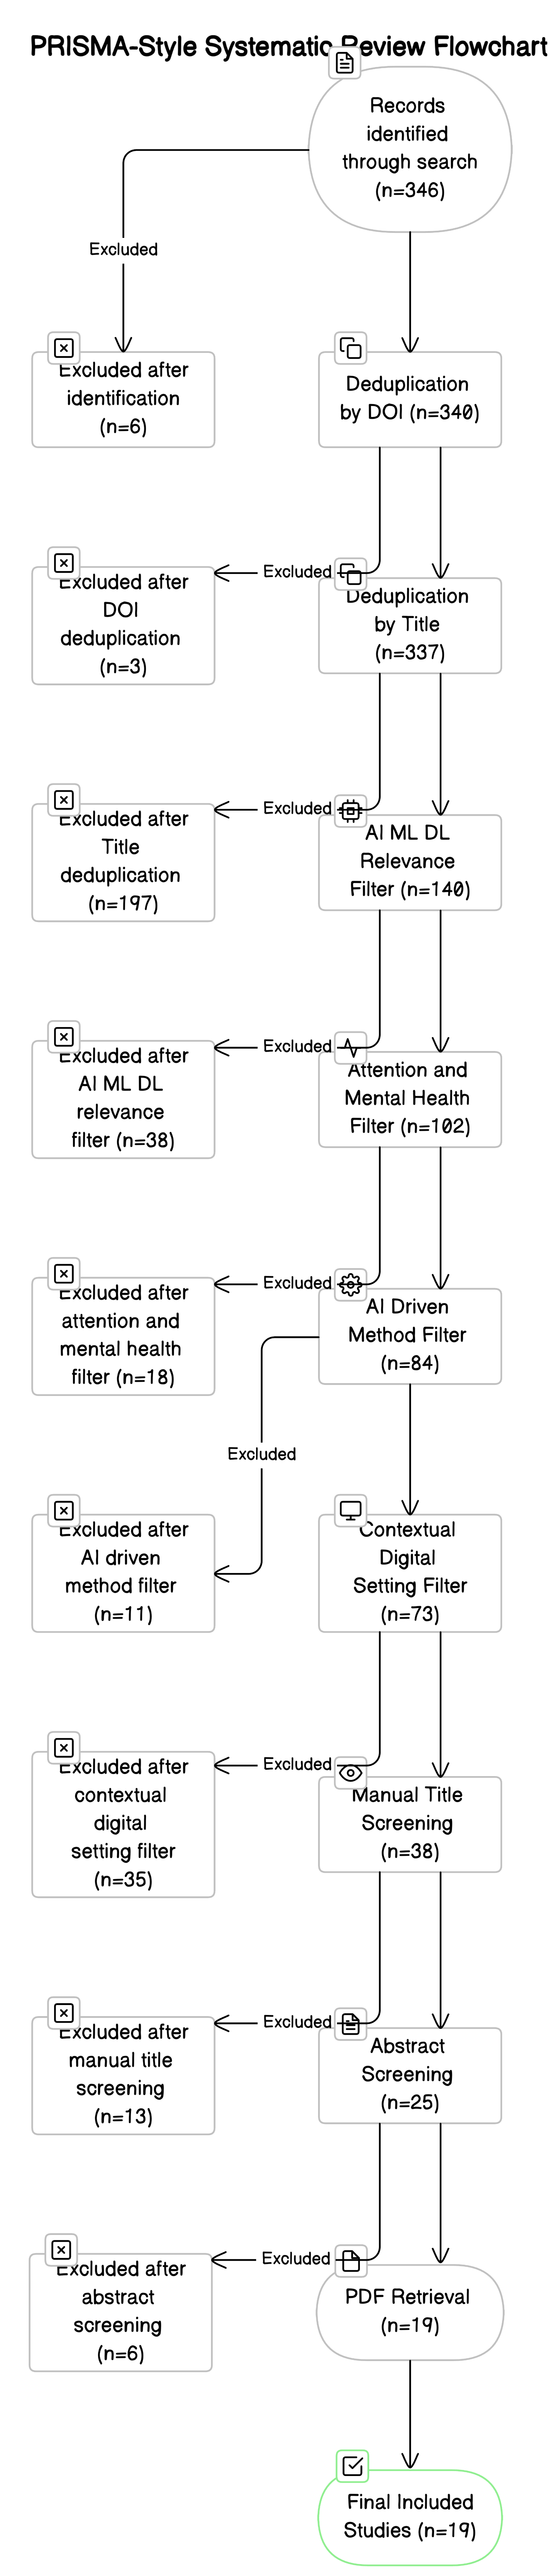
\includegraphics[width=0.27\textwidth]{Prisma.png}
\caption{PRISMA Flowchart}
\end{figure}

\begin{table}[H]
\centering
\hspace{2cm}
\caption{PRISMA Log Table}
\rowcolors{2}{lightgray}{white}
\begin{tabular}{|p{0.50\columnwidth}|p{0.70\columnwidth}|p{0.25\columnwidth}|p{0.20\columnwidth}|}
\hline
\textbf{Stage} & \textbf{Criteria} & \textbf{Included / Excluded} & \textbf{Paper Remaining Count} \\
\hline
Identification & Records identified using search terms across 7 CSV files from 5 databases & Included & 346 \\
\hline
Deduplication (DOI link) & Removed exact duplicates based on 'DOI link' field using Python script & Excluded & 340 \\
\hline
Deduplication (Title) & Removed additional duplicates using normalized 'Paper Title' with Python-based string cleaning and matching & Excluded & 337 \\
\hline
AI, ML, DL Relevance Filter & Filtered titles using Python to retain only papers mentioning AI, ML, or DL (handling hyphens, slashes, punctuation) & Excluded & 140 \\
\hline
Attention \& Mental Health Filter & Filtered papers using Python to include only those mentioning attention, focus, cognitive load, or mental health & Excluded & 102 \\
\hline
AI-Driven Method Filter & Included only papers with AI-method terms (e.g., detection, prediction, modeling) in title using Python & Included & 84 \\
\hline
Contextual/Digital Setting Filter & Included only papers with digital or behavioral context terms (e.g., learning, app, social media, human factors) & Included & 73 \\
\hline
Manual Title Screening & Manually excluded irrelevant papers based on subjective review of titles and topic fit & Excluded & 38 \\
\hline
Abstract Screening & Retained only highly relevant papers after manual review of abstracts against SLR criteria and RQs & Included & 25 \\
\hline
PDF Retrieval & Successfully retrieved full-text PDF versions of selected papers for in-depth review & Included & 19 \\
\hline
\end{tabular}
\end{table}



% Long table: temporarily switch to one column for better fit
\onecolumn
\vspace{1em}
\section{Data Extraction}
This table summarizes key extracted information from 19 reviewed research papers related to AI based attention monitoring, focus, and engagement detection.

\rowcolors{2}{lightgray}{white}

{\scriptsize % smaller font for the entire table
\setlength{\tabcolsep}{3pt}       % reduce horizontal padding (default ~6pt)
\renewcommand{\arraystretch}{0.85} % reduce vertical padding (default 1.0)

\begin{longtable}{|p{0.03\textwidth}|p{0.16\textwidth}|p{0.15\textwidth}|p{0.14\textwidth}|p{0.09\textwidth}|p{0.12\textwidth}|p{0.12\textwidth}|p{0.15\textwidth}|}
\hline
\textbf{No.} & \tablecell{\textbf{Paper Title}} & \tablecell{\textbf{AI Techniques Used}} & \tablecell{\textbf{Dataset Description}} & \tablecell{\textbf{Evaluation Metrics}} & \tablecell{\textbf{Reported Accuracy / Effectiveness}} & \tablecell{\textbf{Key Challenges Noted}} & \tablecell{\textbf{Future Directions Suggested}} \\
\hline
\endfirsthead
\hline
\textbf{No.} & \tablecell{\textbf{Paper Title}} & \tablecell{\textbf{AI Techniques Used}} & \tablecell{\textbf{Dataset Description}} & \tablecell{\textbf{Evaluation Metrics}} & \tablecell{\textbf{Reported Accuracy / Effectiveness}} & \tablecell{\textbf{Key Challenges Noted}} & \tablecell{\textbf{Future Directions Suggested}} \\
\hline
\endhead
1 & \tablecell{Student’s Attention Monitoring System in Learning Environments based on Artificial Intelligence [1]} & \tablecell{YOLO v3, Deep Learning, Computer Vision} & \tablecell{Facial expressions, head pose, motion data from video conferences} & \tablecell{Accuracy, Attention \%, Facial Expression Detection} & \tablecell{High real-time monitoring accuracy} & \tablecell{Real-time performance, virtual learning limitations, facial expression analysis} & \tablecell{Multi-modal learning, real-time behavior analysis, virtual engagement} \\
\hline
2 & \tablecell{Predicting Level of Visual Focus of Human’s Attention Using ML Approaches [2]} & \tablecell{Logistic Regression, SVM, Decision Tree, KNN, AdaBoost, MLP, Extra Tree, Voting Classifier} & \tablecell{Survey reports + eyeball tracking} & \tablecell{Accuracy} & \tablecell{LR: 96\%, Voting: 95\%} & \tablecell{Small sample, self-report bias, simple hardware} & \tablecell{Larger diverse samples, personalization, real-time data} \\
\hline
3 & \tablecell{Classification of EEG Signals for Cognitive Load Estimation Using DL Architectures [3]} & \tablecell{SDAE+MLP, LSTM+MLP, SVM, KNN, LDA} & \tablecell{EEG data (64-channel) at IIT Kharagpur} & \tablecell{Accuracy} & \tablecell{LSTM+MLP: 85.42\%} & \tablecell{Small dataset, subject variability, denoising} & \tablecell{Larger datasets, personalization, hybrid models} \\
\hline
4 & \tablecell{Cognitive Load Estimation Using Hybrid Cluster-Based Unsupervised ML Technique [4]} & \tablecell{Hybrid clustering, 1D CNN} & \tablecell{4-channel wearable EEG (Baseline \& Stroop test)} & \tablecell{Accuracy, Homogeneity, ARI, SC} & \tablecell{Accuracy: 93.2\%, ARI: 0.78} & \tablecell{Generalization, real-world application} & \tablecell{Real-time estimation, low manual effort} \\
\hline
5 & \tablecell{Early Detection of Preschool Children with ADHD Using AI \& Mobile Apps [5]} & \tablecell{Mobile apps, AI tools, video analytics} & \tablecell{Psychometric scales, behavioral data, app usage} & \tablecell{DSM-5/ICD-10, clinical validation} & \tablecell{Mobile apps effective for early detection} & \tablecell{Subjectivity, comorbidity, over/under-diagnosis} & \tablecell{Larger validation, explainable AI, early intervention} \\
\hline
6 & \tablecell{TeacherEye: AI-Powered Monitoring System for Online Education [6]} & \tablecell{DeepFace, VGG-Face, Dlib, MediaPipe, GPT-4} & \tablecell{Webcam video/audio, face images, speech clips} & \tablecell{Recall, WER, Precision} & \tablecell{Face ID: 100\%, Audio: 92.6\%, Cheating: 80\%} & \tablecell{Privacy, false positives, sensory limits} & \tablecell{On-device processing, GUI integration} \\
\hline
7 & \tablecell{Students’ Attention Assessment in eLearning with ML [7]} & \tablecell{Gabor, SVM, NBC, KNN, PCA, facial landmarks} & \tablecell{CEW dataset (eye state), 32x32 pixel images} & \tablecell{Classification Accuracy} & \tablecell{Gabor+SVM: 93.1\%} & \tablecell{Binary classification only, frontal face required} & \tablecell{Blink detection, diverse attention features} \\
\hline
8 & \tablecell{Real-Time Attention Monitoring with DL [8]} & \tablecell{YOLOv5, DeepSORT} & \tablecell{5,701 action images + 35,000 emotion images} & \tablecell{Precision, Recall, mAP@0.5, F1} & \tablecell{Action: 76\% mAP, Emotion: 87.7\% mAP} & \tablecell{Small dataset, privacy} & \tablecell{Multi-modal fusion, explainable AI} \\
\hline
9 & \tablecell{Student-Engagement Detection in Classroom Using ML [9]} & \tablecell{CATBoost, XGBoost, LightGBM} & \tablecell{OULAD dataset (32,593 records)} & \tablecell{Accuracy, F1, AUC-ROC} & \tablecell{CATBoost: 92.23\%, AUC: 0.9626} & \tablecell{Class imbalance} & \tablecell{Adaptive interventions} \\
\hline
10 & \tablecell{Dyslexia Adaptive Learning Model: Engagement Prediction [10]} & \tablecell{SVM, BoF, k-Means} & \tablecell{600 face images (30 students)} & \tablecell{Accuracy} & \tablecell{SVM Linear: 97.8\%} & \tablecell{Small sample, occlusion} & \tablecell{Integrate video} \\
\hline
11 & \tablecell{ML in ADHD and Depression Mental Health Diagnosis: A Survey [11]} & \tablecell{SVM, CNN, Random Forest} & \tablecell{ADHD-200 (973), DAIC-WOZ (142)} & \tablecell{Accuracy, AUC} & \tablecell{ADHD: 99.58\%, Depression: 100\% (EEG)} & \tablecell{Data imbalance} & \tablecell{Multimodal datasets} \\
\hline
12 & \tablecell{ML in ADHD: Neural Mechanism Analysis [12]} & \tablecell{SVM, DNN, LASSO} & \tablecell{ADHD-200, ABCD} & \tablecell{AUC, Sensitivity} & \tablecell{60-90\% Accuracy} & \tablecell{Small samples} & \tablecell{Generative models} \\
\hline
13 & \tablecell{Automatic Diagnosis of ADHD Using ML [13]} & \tablecell{Decision Tree, Random Forest, SVM} & \tablecell{NHS data (69 patients)} & \tablecell{AUC} & \tablecell{DT: 85.5\%, AUC: 0.871} & \tablecell{Overfitting} & \tablecell{Fuzzy rule-based models} \\
\hline
14 & \tablecell{Game Data Analysis for ADHD Assessment [14]} & \tablecell{AdaBoost, JRip} & \tablecell{Sifteo Cubes, 52 subjects} & \tablecell{F-measure} & \tablecell{75-78\% Accuracy} & \tablecell{Hardware limits} & \tablecell{Neuroplasticity integration} \\
\hline
15 & \tablecell{ADHD Detection Using Multimodal Physiological Data [15]} & \tablecell{SVM, Random Forest} & \tablecell{76 adults} & \tablecell{Accuracy} & \tablecell{SVM: 81.6\%} & \tablecell{No comorbidity control} & \tablecell{Larger validations} \\
\hline
16 & \tablecell{Autism Spectrum Disorder Assessment Using ML [16]} & \tablecell{LSTM, CNN, SVM} & \tablecell{Eye-tracking datasets} & \tablecell{AUC} & \tablecell{Up to 93.7\% (SVM)} & \tablecell{Ecological validity} & \tablecell{VR tool integration} \\
\hline
17 & \tablecell{ML on Psychometric Questionnaires for ADHD [17]} & \tablecell{12+ ML techniques} & \tablecell{35–13,000 participants} & \tablecell{AUC} & \tablecell{AUC: 0.56–0.992} & \tablecell{Subjectivity} & \tablecell{Multi-informant model} \\
\hline
18 & \tablecell{ADHD Identification with Deep Learning [18]} & \tablecell{BiLSTM, MVMD} & \tablecell{121-subject EEG data} & \tablecell{ROC-AUC} & \tablecell{Accuracy: 95.54\%} & \tablecell{EEG artifacts} & \tablecell{Real-time system} \\
\hline
19 & \tablecell{ADHD Diagnosis Using SPECT with ML [19]} & \tablecell{SVM, KNN} & \tablecell{236 brain scans} & \tablecell{F-measure} & \tablecell{Accuracy: 98\%} & \tablecell{Class imbalance} & \tablecell{Subtype classification} \\
\hline
\end{longtable}
\twocolumn

\section{Results}
This section represents an analysis of what we found from the 19 reviewed papers. We analyze the paper on the basis of some questions related to Artificial Intelligence techniques, datasets, evaluation metrics, effectiveness, challenges, and future directions in Artificial Intelligence based attention assessment.

\subsection{What Artificial Intelligence techniques are commonly used for assessing attention and focus in digital environments?}
From the reviewed papers, a large range of Artificial Intelligence techniques were used to assess attention and focus, advancements in machine learning, and deep learning. These methods were applied to different datasets, such as physiological signals (such as, \textbf{EEG}), behavioral data (such as, \textbf{facial expressions}, \textbf{eye-tracking}), and environmental factors (such as, \textbf{video data from classrooms}).

\begin{itemize}
    \item \textbf{Deep Learning Models}: Deep learning methods, especially Convolutional \textbf{Neural Networks (CNNs)} and \textbf{Long Short-Term Memory (LSTM)} networks, were frequently used for attention and focus detection tasks involving sequential or image data. As an example, \textbf{YOLOv3} and \textbf{YOLOv5} Papers~([\citealp{ref1}], [\citealp{ref8}]) were used to analyze real-time student behavior in classrooms and e-Learning environments. These models can have significant effectiveness in detecting attention by tracking facial expressions and body movements.
    \item \textbf{Support Vector Machines (SVM)}: \textbf{SVM} was another widely used method, especially for classification tasks involving \textbf{EEG} and \textbf{behavioral data}. SVM models were found to perform well in identifying attention-based patterns and cognitive states, especially in \textbf{ADHD} diagnosis and cognitive load estimation tasks Papers~([\citealp{ref11}], [\citealp{ref12}], [\citealp{ref19}]). Combining with methods like \textbf{Random Forest} or \textbf{Deep Neural Networks (DNNs)} the SVM classifiers can have high accuracy in detecting attention shifts.
    \item \textbf{Random Forest and Ensemble Methods}: \textbf{Random Forest}, \textbf{AdaBoost}, and \textbf{XGBoost} were used in various studies for tasks such as classifying attention in educational factors and diagnosing \textbf{ADHD}. These models provided robust results by combining multiple classifiers but small sample sizes cause overfitting Papers~([\citealp{ref2}], [\citealp{ref13}], [\citealp{ref15}]).
    \item \textbf{Behavioral and Physiological Data Integration}: An important section that the integration of multiple data types, such as \textbf{facial expression recognition (FER)}, \textbf{eye-tracking}, and \textbf{EEG data}. The integration of these features using machine learning techniques like \textbf{SVM} or \textbf{Deep Neural Networks (DNNs)} allowed for better prediction of attention levels Papers~([\citealp{ref7}], [\citealp{ref16}]). This combination of data types made the models stronger by balancing out the weaknesses.
\end{itemize}

\begin{figure}[H]
\centering
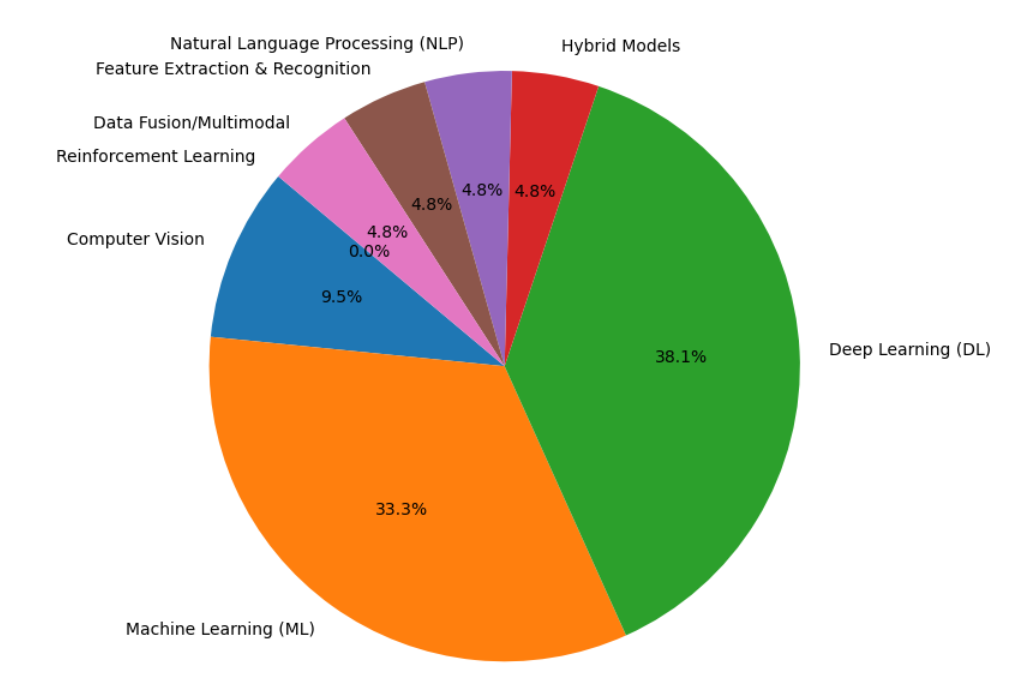
\includegraphics[width=0.5\textwidth]{piechart.png}
\caption{Distribution of AI Techniques Used}
\label{fig:piechart}
\end{figure}

\vspace{1em} % small vertical space between figure and table

\begin{table}[H]
\centering
\footnotesize               % smaller font size
\setlength{\tabcolsep}{2pt} % reduce horizontal padding (default ~6pt)
\renewcommand{\arraystretch}{.5} % reduce vertical row spacing (default 1.0)
\caption{AI Subfields and Techniques Summary}
\rowcolors{2}{lightgray}{white}
\begin{tabular}{|p{2cm}|p{3cm}|p{1.5cm}|p{2.5cm}|}
\hline
\textbf{AI Subfield} & \textbf{Techniques Used} & \textbf{Number of Papers} & \textbf{Paper Numbers} \\
\hline
Computer Vision & YOLO v3, Deep Learning, Computer Vision & 2 & Papers~([\citealp{ref1}], [\citealp{ref8}]) \\
\hline
Machine Learning (ML) & Logistic Regression, SVM, Decision Tree, KNN, AdaBoost, MLP, Extra Tree Classifier, Voting Classifier & 7 & Papers~([\citealp{ref2}], [\citealp{ref3}], [\citealp{ref7}], [\citealp{ref9}], [\citealp{ref10}], [\citealp{ref12}], [\citealp{ref13}]) \\
\hline
Deep Learning & SDAE + MLP, LSTM + MLP, 1D CNN, CNN, BiLSTM, DNN & 8 & Papers~([\citealp{ref3}], [\citealp{ref4}], [\citealp{ref6}], [\citealp{ref8}], [\citealp{ref11}], [\citealp{ref12}], [\citealp{ref18}], [\citealp{ref19}]) \\
\hline
Hybrid Models & Hybrid cluster-based unsupervised learning, 1D CNN & 1 & Paper~([\citealp{ref4}]) \\
\hline
Natural Language Processing (NLP) & Whisper API, GPT-4 & 1 & Paper~([\citealp{ref6}]) \\
\hline
Feature Extraction \& Recognition & DeepFace, VGG-Face, Dlib, EAR, MobileNet-SSD, MediaPipe Pose, FER & 1 & Paper~([\citealp{ref6}]) \\
\hline
Data Fusion/Multimodal & Multiple ML techniques (integrated analysis across modalities) & 1 & Paper~([\citealp{ref7}]) \\
\hline
Reinforcement Learning & None & 0 & - \\
\hline
\end{tabular}
\label{tab:ai_subfields}
\end{table}


\subsection{What datasets and evaluation metrics are used for Artificial Intelligence based attention assessment studies?}
The datasets and evaluation metrics used in the reviewed studies varied greatly, reflecting the differences in attention-related tasks. From diagnostic assessments of different datasets and metrics were used to monitoring attention in real-time classroom factors and attention disorders like ADHD. \\ \\
\textbf{Datasets:} A range of datasets was applied to assess attention and focus, with a focus on both behavioral data and physiological signals. \\ \\
\textbullet \textbf{EEG-based datasets} were most commonly used in the context of cognitive load and attention deficit detection.  For example, the \textbf{ADHD-200} dataset gave a large collection of EEG data for ADHD classification Papers~([\citealp{ref11}], [\citealp{ref19}]). Also, EEG data from wearable devices were used in real-time attention estimation tasks Papers~([\citealp{ref3}], [\citealp{ref4}]).  \\ \\
\textbullet \textbf{Eye-tracking datasets} were also common in attention studies, especially for analyzing visual attention in e-Learning and classroom environments. The \textbf{CEW dataset} and \textbf{OULAD dataset} gave data on eye states, facial expressions and pupil movements. Papers~([\citealp{ref7}], [\citealp{ref9}]).  \\ \\ \\
\textbullet \textbf{SPECT brain scans} were used in some studies to assess brain activity and its correlation with attention deficits Paper~([\citealp{ref19}]). These datasets used for understanding attention-related disorders in-depth.  \\ \\
\textbullet \textbf{Facial expression datasets} were generally useful in assessing attention in facial expressions were linked to students' engagement levels Papers~([\citealp{ref1}], [\citealp{ref9}]).  \\ \\

\textbf{Evaluation Metrics:} Several evaluation metrics were used to assess the effectiveness of Artificial Intelligence models in detecting attention shifts and disorders:  \\ \\
\textbullet \textbf{Accuracy} was the most common metric that is used to classifying attention levels in real-time systems Papers~([\citealp{ref1}], [\citealp{ref3}], [\citealp{ref8}]). \textbf{Deep Learning} and \textbf{SVM} models achieved high accuracy scores in various attention-related tasks.  \\ \\
\textbullet \textbf{Precision, Recall, and F1-Score} were commonly used to evaluate performance in imbalanced datasets, that in real-time applications where precision and recall are important for identifying both attention and distraction states Papers~([\citealp{ref2}], [\citealp{ref6}], [\citealp{ref9}]).  \\ \\
\textbullet \textbf{Area Under Curve (AUC)} was often used for ADHD detection and cognitive load estimation tasks. Those observed in studies with \textbf{SVM} Papers~([\citealp{ref11}], [\citealp{ref12}], [\citealp{ref19}]), which has High AUC values, demonstrated the ability of model that discriminates between different attention-related states effectively.  \\ \\
\textbullet \textbf{Homogeneity Score} and \textbf{Silhouette Coefficient} were used in unsupervised learning models to assess the quality of clustering in attention data Paper~([\citealp{ref4}])).  \\ 

\subsection{How effective are machine learning models in detecting shifts in attention?} 
The machine learning models demonstrated varying levels of effectiveness depending on the dataset used and the context of the task: \\ 

\textbullet \textbf{Real-Time Attention Monitoring:} It is used for monitoring attention in classroom and e-Learning environments, \textbf{Deep Learning} models such as \textbf{YOLOv3} and \textbf{YOLOv5} work brilliantly in real-time performance, detecting attention shifts with high accuracy Paper~([\citealp{ref8}]). These models were capable of processing video data to assess facial expressions and body movements, which are the main indicators of attention in educational settings. \\ \\ 
\textbullet \textbf{EEG and Cognitive Load Estimation:} Deep learning models like \textbf{SDAE + MLP} and \textbf{LSTM + MLP} achieved accuracies of up to \textbf{85.42\%} for detecting shifts in cognitive load and attention using EEG Paper~([\citealp{ref3}]). These models were effective in detecting subtle shifts in attention during tasks of varying difficulty and also highlighting their potential in cognitive workload management.  \\ \\
\textbullet \textbf{ADHD Detection:} \textbf{ADHD-200} and \textbf{SPECT brain scans} were highly effective in detecting attention deficits associated with \textbf{ADHD} that achieving accuracies of \textbf{up to 99.58\%} Papers~([\citealp{ref11}], [\citealp{ref19}]). All of these models used a combination of \textbf{SVM}, \textbf{Random Forest}, and \textbf{CNN} architectures to classify \textbf{ADHD} based on neuroimaging and physiological data.  \\ \\
\textbullet \textbf{Facial Expression and Eye-Tracking Models:} Models analyzing facial expressions and eye-tracking data in classroom settings demonstrated high performance that accuracies ranging \textbf{from 85\% to 93.1\%} Papers~([\citealp{ref7}], [\citealp{ref8}]). These models were especially effective at detecting attention shifts which is related to student engagement in educational contexts.  \\ 

\subsection{Challenges and Limitations in Artificial Intelligence-Powered Attention Assessment}

Several challenges and limitations were identified across the reviewed studies:

\begin{itemize}
    \item \textbf{Data-Related Issues:} Many studies suffered from \textbf{small sample sizes}~\citep{ref3,ref13}. Additionally, \textbf{data imbalance} was a significant issue in datasets involving attention states, where low-attention states were often underrepresented~\citep{ref9,ref19}.
    
    \item \textbf{Overfitting:} Overfitting was a common problem in models trained on small or highly specific datasets, leading to reduced performance on unseen data~\citep{ref6,ref15}.
    
    \item \textbf{Privacy and Ethical Concerns:} The use of \textbf{biometric data}, including facial expressions, EEG, and physiological measurements, raised important privacy and ethical issues, especially when working with children~\citep{ref6,ref15}.
    
    \item \textbf{Hardware Constraints:} Many models required specialized equipment such as \textbf{EEG headsets} and \textbf{eye-trackers}, limiting scalability in real-world applications. Developing models less reliant on expensive hardware remains a key challenge~\citep{ref8,ref14}.
\end{itemize}

\begin{table}[H]
\centering
\footnotesize
\setlength{\tabcolsep}{1pt}
\renewcommand{\arraystretch}{1.5}
\caption{Key Limitations Identified in Reviewed Papers}
\rowcolors{2}{lightgray}{white}
\begin{tabular}{|p{0.16\textwidth}|p{0.16\textwidth}|p{0.16\textwidth}|}
\hline
\textbf{Key Limitation} & \textbf{No. of Papers Addressing 
Limitation} & \textbf{Papers} \\
\hline
Small sample size & 8 & Papers~\citep{ref2,ref3,ref4,ref7,ref10,ref12,ref14,ref15} \\
\hline
Data imbalance & 3 & Papers~\citep{ref9,ref11,ref13} \\
\hline
Subject variability & 1 & Paper~\citep{ref3} \\
\hline
Privacy concerns & 2 & Papers~\citep{ref6,ref8} \\
\hline
Overfitting risk & 1 & Paper~\citep{ref13} \\
\hline
Comorbidities and diagnosis accuracy & 2 & Papers~\citep{ref5,ref15} \\
\hline
Limited feature sets (e.g., blink frequency, eye states) & 2 & Papers~\citep{ref7,ref8} \\
\hline
Lack of ecological validity (real-world applicability) & 1 & Paper~\citep{ref16} \\
\hline
No control for confounding factors (e.g., comorbidities) & 1 & Paper~\citep{ref15} \\
\hline
\end{tabular}
\end{table}

\subsection{Future Research Directions for Artificial Intelligence-Based Attention Analysis}

The reviewed studies suggest several important directions for advancing AI-based attention assessment:

\begin{itemize}
    \item \textbf{Multimodal Approaches:} Combining multiple data types such as \textbf{EEG}, \textbf{facial expressions}, and \textbf{eye-tracking} to improve attention detection accuracy. Multimodal systems reduce the limitations of individual data types and create more robust models~\citep{ref1,ref7,ref8}.
    
    \item \textbf{Real-Time Systems and Scalability:} Developing \textbf{real-time attention monitoring systems} suitable for dynamic environments like classrooms or workplaces. Enhancing scalability to handle larger, diverse populations will strengthen model robustness~\citep{ref6,ref16}.
    
    \item \textbf{Explainability and Transparency:} Integrating \textbf{explainable Artificial Intelligence (XAI)} methods to ensure transparency and understandability, especially critical in clinical applications like ADHD diagnosis~\citep{ref10,ref19}.
    
    \item \textbf{Larger Datasets and Personalized Models:} Expanding datasets to include diverse populations and contexts will improve generalizability. Personalized models that adapt to individual cognitive processing are encouraged to enhance system effectiveness~\citep{ref5,ref9}.
    
    \item \textbf{Integration with Educational Tools:} Embedding AI attention monitoring with \textbf{e-Learning platforms} and \textbf{virtual reality tools} to provide real-time feedback and personalized support, thereby enhancing student engagement and learning outcomes~\citep{ref7,ref8}.
\end{itemize}

\begin{figure}[H]
\centering
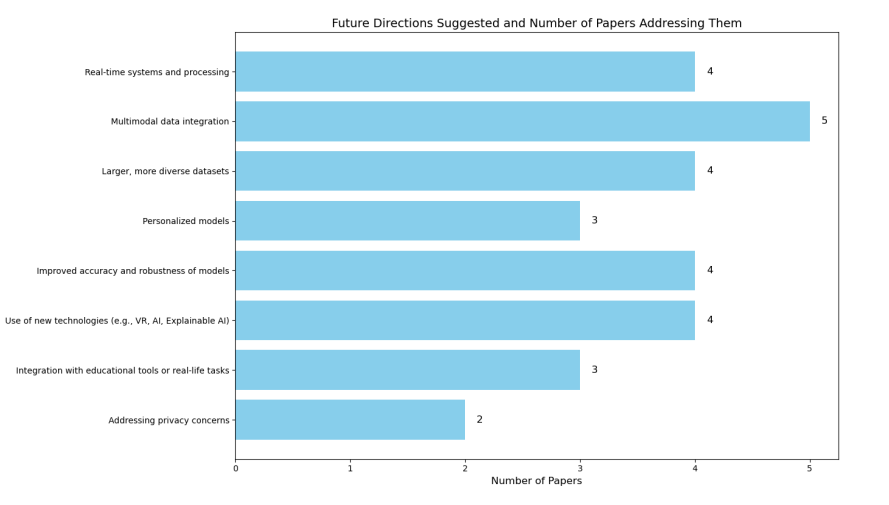
\includegraphics[width=0.6\textwidth]{bar.png}
\caption{Future Directions Suggested by Papers}
\end{figure}

\begin{table}[H]
\centering
\footnotesize
\setlength{\tabcolsep}{1pt}
\renewcommand{\arraystretch}{0.5}
\caption{Future Research Directions Identified in Reviewed Papers}
\rowcolors{2}{lightgray}{white}
\begin{tabular}{|p{0.16\textwidth}|p{0.16\textwidth}|p{0.16\textwidth}|}
\hline
\textbf{Future Direction Suggested} & \textbf{No. of Papers Addressing Suggestion} & \textbf{Papers} \\
\hline
Real-time systems and processing & 4 & Papers~\citep{ref1,ref3,ref4,ref18} \\
\hline
Multimodal data integration & 5 & Papers~\citep{ref2,ref5,ref8,ref11,ref15} \\
\hline
Larger, more diverse datasets & 4 & Papers~\citep{ref2,ref3,ref5,ref11} \\
\hline
Personalized models & 3 & Papers~\citep{ref2,ref3,ref5} \\
\hline
Improved accuracy and robustness of models & 4 & Papers~\citep{ref5,ref6,ref9,ref17} \\
\hline
Use of new technologies (e.g., VR, AI, Explainable AI) & 4 & Papers~\citep{ref1,ref5,ref6,ref16} \\
\hline
Integration with educational tools or real-life tasks & 3 & Papers~\citep{ref1,ref6,ref7} \\
\hline
Addressing privacy concerns & 2 & Papers~\citep{ref6,ref8} \\
\hline
\end{tabular}
\end{table}

\section{Discussion}
In this section, we explore what the systematic literature review reveals about Artificial Intelligence powered methods for assessing attention and focus in digital age. We connect the main findings to existing research and also analyze at the strengths and weaknesses of the different approaches that were reviewed.

\subsection{ Artificial Intelligence Techniques for Assessing Attention} \\

It is evident from the review that many types of Artificial Intelligence have been successfully employed.
It is applied to gauge how much attention users pay to online content. Starting with advanced deep learning models like
\textbf{YOLOv3}, \textbf{YOLOv5}, and LSTM are sieved down to more well-known techniques such as \textbf{SVM} and \textbf{Random Forest} machine learning algorithm. Unstructured data is relatively easy to handle using deep learning models.They can process data, for instance, AI models, with video and physiological signals, unlike conventional models by including readings from EEG and behavioral patterns.
There is a noticeable shift toward multimodal Artificial Intelligence on these papers. Devices collecting information from \textbf{EEG}, \textbf{eye movements}, and \textbf{facial analysis} are linked to give better results expression analysis. These approaches are achieving better outcomes than using just one approach a single dataset. We then connected EEG to face recognition, for example, is an effective method. It allows a more precise measurement of attention and focus and other attention and focus related elements by picking up both the behavior and the mental signals. This leads us to a significant conclusion from the study, which is capable of handling different situations Papers~([\citealp{ref1}], [\citealp{ref7}], [\citealp{ref16}]).

Artificial Intelligence can quickly notice when a person looks away while watching something. Educational settings can be really enjoyable. Technologies such as \textbf{YOLOv5} and  \textbf{DeepSORT} are aiming to help teachers monitor how engaged students are during lessons. Students can attend classes either in person or online. Such improvements are crucial in solving the problem how earlier methods for detecting attention often demanded intrusive techniques equipment.

\subsection{ Dataset Diversity and Evaluation Metrics} \\

The review highlights the use of a wide selection of datasets from various sources datasets made up of studies on \textbf{EEG}, \textbf{facial expressions}, and \textbf{eye tracking}. This variety it shows that attention is difficult to grasp and depends on several kinds of information suitable for different circumstances. Researchers have widely used \textbf{EEG} data in a variety of studies. Studies have shown that both \textbf{SVM} and \textbf{Random Forest} help tackle the problem of cognitive load and \textbf{ADHD}. They have high accuracy in finding attention deficits, as shown in Papers~([\citealp{ref11}], [\citealp{ref19}]). However, a key issue is this still leaves the concern about how small the datasets are in terms of accuracy. These studies can be applied to larger groups of people.

Most analyses measured how well models performed using measurements such as \textbf{accuracy} and \textbf{precision} and \textbf{AUC}. For models aimed at \textbf{ADHD} diagnosis, \textbf{AUC} is particularly significant in research studies Papers~([\citealp{ref11}], [\citealp{ref19}]). Still, the main focus on accuracy as the main measure raises some concerns stops, which are especially critical in cases where datasets have significant imbalance.
This dataset does not have an equal number of high and low attention cases. To make models more accurate during evaluation, researchers should examine other, more advanced measures such as the \textbf{F1-score} or \textbf{balanced}, \textbf{accuracy}. Such metrics give a good idea of how well the model functions.
In practice, datasets often have an imbalance between positive and negative examples.

\subsection{ Effectiveness of Machine Learning Models} \\

Many papers have highlighted that deep learning models offer a strong advantage in machine learning. They are highly successful in noticing changes in someone’s attention, with some showing impressive results. The findings of Hosseini and colleagues were confirmed in real-time applications Papers~([\citealp{ref1}], [\citealp{ref8}]). Models often depend on their performance depending on the type of data being used. For instance, assessing attention in visual tasks usually gives better results when using \textbf{facial expression} and \textbf{eye tracking} techniques. Examining \textbf{EEG} data is better at noticing both cognitive load and declines in attention Reference sources used Papers~([\citealp{ref3}], [\citealp{ref16}]). Combining various elements into one model could be the future of machine intelligence they bring together various sources of data. These approaches help to overcome the constraints faced by single models. It includes methods that provide a better understanding of how a person pays attention how the data is presented. Clinical research suggests that \textbf{EEG-based} models are particularly useful for making diagnoses \textbf{ADHD}. Using \textbf{SVM} and \textbf{Random Forest} models, researchers managed to achieve dramatic results. Some studies reported a level of 99.58\% in recognizing the attention patterns associated with \textbf{EEG}ADHD. Such as Papers~([\citealp{ref11}], [\citealp{ref19}]). According to these findings, AI might be very helpful for these problems. The tool aims to speed up and enhance the diagnostic process by being both quicker and more intelligent. There are better ways to do the task than what is traditionally done. Yet, there are still difficulties to resolve addressed. Struggles like unequal data split, models that learn the information too well, and individual patterns are examples of issues.

\subsection{ Challenges and Limitations} \\ 

Artificial intelligence in attention assessment is seeing some improvement, but may still not be perfect. It faces various ongoing issues. An important limitation is the size of the sample. Mostly of these datasets are created to analyze clinical situations, for example, \textbf{ADHD} and mood disorders Papers~([\citealp{ref11}], [\citealp{ref13}]). Having only a small number of examples can make the data fit the model too much. When the model behaves as it should. When a model performs well when training but fails to give correct results on new data, it is called overfitting. The lack of substantial, quality datasets adds to this challenge. Without
A lot of data that is both broad and inclusive makes it challenging to develop a model that can generalize well. It is effective for various groups of people. There are major concerns about privacy when building Artificial Intelligence.
devices for evaluating attention. Processing facial and eye movement data with AI is simple. Meanwhile, EEG signals pose ethical questions about what to do with personal brain data.
collected, preserved, and used. It is important for people to trust these systems deal with laws related to data privacy such as the \textbf{GDPR}. It is subjective in some cases, information such as self-reports of attention or visual observations which are not completely reliable reflect accurately how someone is thinking about an issue Papers~([\citealp{ref5}], [\citealp{ref6}]).

Making Artificial Intelligence accessible to all is a major concern for developers. Systems that monitor attention. Several models today still require specialized hardware to work efficiently. Just like \textbf{EEG} headsets and \textbf{eye-tracking} devices, which tend to be expensive and difficult to operate. High-end equipment is required, so it can be tricky to carry out in the industry. This happens when resources are limited and the desired application requires processing a larger number of items Papers~([\citealp{ref8}], [\citealp{ref14}]). How can I direct attention to a certain place? To make monitoring technologies more inclusive and practical, new ideas are needed, improve user experience and lower the need for specialized hardware.

\subsection{ Future Research Directions} \\

In the future, there are promising opportunities for Artificial Intelligence to develop attention assessment. A promising trend is the advancement of multimodal. Systems that combine information from EEG readings and expressions are being developed including eye expressions. They are designed to aid in understanding attention better. Integrating can address a lot of the disadvantages that single-modality models often have. From the list I provided, there are several papers in different formats  Papers~([\citealp{ref1}], [\citealp{ref7}]).

Another key focus for future research is \textbf{creating real-time monitoring systems} that can work effectively and smoothly in everyday environments like classrooms or workplaces. Such systems could deliver immediate feedback and enable personalized interventions based on attention levels of a person and ultimately supporting better learning outcomes and improved productivity Papers~([\citealp{ref6}], [\citealp{ref8}]).

\textbf{Incorporating explainable Artificial Intelligence (XAI)} techniques is becoming increasingly important for improving the transparency and trustworthiness of Artificial Intelligence driven attention monitoring systems. It is needed in especially in clinical contexts, where decisions can have significant consequences for an individual health and well-being Papers~([\citealp{ref10}], [\citealp{ref19}])

Additionally, future research should prioritize expanding datasets to include more diverse populations and real-world environments. Larger and more representative data will help build models that are not only more robust but also more generalizable across different population, demographics and use cases Papers~([\citealp{ref9}], [\citealp{ref16}]). This step is essential for developing attention assessment tools that are fair, reliable, and effective in a wider range of settings and sectors.


\section{Conclusion}

Artificial Intelligence-powered approaches to attention assessment have shown remarkable progress, especially in educational and clinical settings. By leveraging advancements in machine learning alongside varied data sources such as \textbf{EEG signals}, \textbf{facial expressions}, and \textbf{eye-tracking}, researchers have been able to effectively detect attention shifts and support the diagnosis of attention-related disorders.

Despite these advancements, challenges remain including \textbf{limited sample sizes}, \textbf{data privacy concerns}, and \textbf{dependence on specialized hardware}, which affect broader adoption. Future research should prioritize building generalizable models, expanding datasets with diverse populations, and advancing multimodal systems. These steps will contribute to making AI-powered attention assessment tools more accurate, ethical, and applicable to real-world scenarios.

\vspace{1em}

\section*{References}
\begingroup
\setlength{\parskip}{0.4em}
\setlength{\itemsep}{0pt}
\renewcommand{\section}[2]{}%
\begin{thebibliography}{99}

\bibitem{ref1} D. F. Terraza Arciniegas, M. Amaya, A. Piedrahita Carvajal, P. A. Rodriguez-Marin, L. Duque-Muñoz, and J. D. Martinez-Vargas, “Students’ Attention Monitoring System in Learning Environments based on Artificial Intelligence,” \textit{IEEE Latin America Transactions}, vol. 20, no. 1, pp. 126–132, Jan. 2022, doi: 10.1109/TLA.2022.9662181.

\bibitem{ref2} P. Chakraborty, M. A. Yousuf, and S. Rahman, “Predicting Level of Visual Focus of Human’s Attention Using Machine Learning Approaches,” in \textit{Proc. Int. Conf. Trends Comput. Cogn. Eng.}, Springer, Singapore, 2021, vol. 1309, doi: 10.1007/978-981-33-4673-4\_56.

\bibitem{ref3} A. Saha, V. Minz, S. Bonela, S. R. Sreeja, R. Chowdhury, and D. Samanta, “Classification of EEG Signals for Cognitive Load Estimation Using Deep Learning Architectures,” in \textit{Intelligent Human Computer Interaction (IHCI 2018)}, vol. 11278, Springer, Cham, 2018, doi: 10.1007/978-3-030-04021-5\_6.

\bibitem{ref4} I. Hassan, M. Zolezzi, H. Khalil, R. M. Al Saady, S. Pedersen, and M. E. H. Chowdhury, “Cognitive Load Estimation Using a Hybrid Cluster-Based Unsupervised Machine Learning Technique,” \textit{IEEE Access}, vol. 12, pp. 118785–118801, 2024, doi: 10.1109/ACCESS.2024.3428691.

\bibitem{ref5} V. Tsakou and A. Drigas, “Early Detection of Preschool Children with ADHD and the role of mobile Apps and AI,” \textit{Technium Social Sciences Journal}, vol. 30, no. 1, pp. 127–137, 2022, doi: 10.47577/tssj.v30i1.6266.

\bibitem{ref6} Z. Abdelhadi, M. Naseif, W. Alhejali, and A. Elhayek, “TeacherEye: An AI-Powered System for Monitoring Student Engagement in Online Education,” in \textit{Proc. 22nd Int. Learn. Technol. Conf. (L\&T)}, Jeddah, Saudi Arabia, 2025, pp. 25–30, doi: 10.1109/LT64002.2025.10940905.

\bibitem{ref7} Q. Deng and Z. Wu, “Untitled,” \textit{IOP Conf. Ser.: Earth Environ. Sci.}, vol. 199, p. 032042, 2018, doi: 10.1088/1755-1315/199/3/032042.

\bibitem{ref8} Z. Trabelsi, F. Alnajjar, M. M. A. Parambil, M. Gochoo, and L. Ali, “Real-Time Attention Monitoring System for Classroom: A Deep Learning Approach for Student’s Behavior Recognition,” \textit{Big Data Cogn. Comput.}, vol. 7, p. 48, 2023, doi: 10.3390/bdcc7010048.

\bibitem{ref9} N. Alruwais and M. Zakariah, “Student-Engagement Detection in Classroom Using Machine Learning Algorithm,” \textit{Electronics}, vol. 12, p. 731, 2023, doi: 10.3390/electronics12030731.

\bibitem{ref10} S. S. Abdul Hamid, N. Admodisastro, N. Manshor, A. Kamaruddin, and A. A. A. Ghani, “Dyslexia Adaptive Learning Model: Student Engagement Prediction Using Machine Learning Approach,” in \textit{Recent Advances on Soft Computing and Data Mining (SCDM 2018)}, vol. 700, Springer, Cham, 2018, doi: 10.1007/978-3-319-72550-5\_36.

\bibitem{ref11} C. Nash, R. Nair, and S. M. Naqvi, “Machine Learning in ADHD and Depression Mental Health Diagnosis: A Survey,” \textit{IEEE Access}, vol. 11, pp. 86297–86317, 2023, doi: 10.1109/ACCESS.2023.3304236.

\bibitem{ref12} M. Cao, E. Martin, and X. Li, “Machine learning in attention-deficit/hyperactivity disorder: new approaches toward understanding the neural mechanisms,” \textit{Transl Psychiatry}, vol. 13, p. 236, 2023, doi: 10.1038/s41398-023-02536-w.

\bibitem{ref13} T. Chen, G. Antoniou, M. Adamou, I. Tachmazidis, and P. Su, “Automatic Diagnosis of Attention Deficit Hyperactivity Disorder Using Machine Learning,” \textit{Applied Artificial Intelligence}, vol. 35, no. 9, pp. 657–669, 2021, doi: 10.1080/08839514.2021.1933761.

\bibitem{ref14} M. D. Heller, K. Roots, S. Srivastava, J. Schumann, J. Srivastava, and T. S. Hale, “A Machine Learning-Based Analysis of Game Data for Attention Deficit Hyperactivity Disorder Assessment,” \textit{Games for Health Journal}, vol. 2, no. 5, pp. 291–298, 2013, doi: 10.1089/g4h.2013.0058.

\bibitem{ref15} D. Andrikopoulos, G. Vassiliou, P. Fatouros et al., “Machine learning-enabled detection of attention-deficit/hyperactivity disorder with multimodal physiological data: a case-control study,” \textit{BMC Psychiatry}, vol. 24, p. 547, 2024, doi: 10.1186/s12888-024-05987-7.

\bibitem{ref16} M. E. Minissi, I. A. Chicchi Giglioli, F. Mantovani et al., “Assessment of the Autism Spectrum Disorder Based on Machine Learning and Social Visual Attention: A Systematic Review,” \textit{J Autism Dev Disord}, vol. 52, pp. 2187–2202, 2022, doi: 10.1007/s10803-021-05106-5.

\bibitem{ref17} L. Caselles-Pina, A. Quesada-López, A. Sújar, E. M. Garzón Hernández, and D. Delgado-Gómez, “A systematic review on the application of machine learning models in psychometric questionnaires for the diagnosis of attention deficit hyperactivity disorder,” \textit{Eur. J. Neurosci.}, vol. 60, no. 3, pp. 4115–4127, 2024, doi: 10.1111/ejn.16288.

\bibitem{ref18} Ö. Kasim, “Identification of attention deficit hyperactivity disorder with deep learning model,” \textit{Phys. Eng. Sci. Med.}, vol. 46, pp. 1081–1090, 2023, doi: 10.1007/s13246-023-01275-y.

\bibitem{ref19} M. de O. Meira, A. M. de P. Canuto, B. M. de Carvalho, and R. L. C. Jales, “Comparison of Machine Learning predictive methods to diagnose the Attention Deficit/Hyperactivity Disorder levels using SPECT,” \textit{Research, Society and Development}, vol. 11, no. 8, p. e54811831258, 2022, doi: 10.33448/rsd-v11i8.31258.

\end{thebibliography}
\endgroup

\end{document}
